\section{Server Security}

Man sollte immer davon ausgehen, dass die verwendete Software Schwachstellen besitzt. Auch wenn diese Schwachstellen vielleicht nicht ausreichen, können sie dennoch als Sprungbrett für andere Angriffe verwendet werden. Daher ist es zwingend notwendig, das System auf allen möglichen Ebenen zu sichern (\textbf{Hardening}). Man spricht dabei von einer \textbf{Multi-Defense Strategy}.\\

Statistisch gesehen existiert für eine neu entdeckte Sicherheitslücke nach \textbf{6 Tagen ein Exploit} und erst \textbf{nach 54 Tagen ein Patch}. Oftmals ist bereits der Lesezugriff ausreichend, um einem Unternehmen Schaden zuzufügen oder daraus zu profitieren. Besitzt der Angreifer noch Schreibzugriff, so kann er Anwendungen auf den Server laden und diese später ausführen. Beispiel: \textit{PHP Shell}.

\subsection{Ziele der Angreifer}
\begin{enumerate}
	\item \textbf{Read} files from the server (e.g. \textit{XXE File Inclusion})
	\item \textbf{Write} files to the server (e.g. JSP-, PHP-, DLL-Files)
	\item \textbf{Execute}
	\subitem commands (exploit contains command)
	\subitem server commands (e.g. cmd.exe)
	\subitem uploaded files on server (e.g. phpshell)
	\item \textbf{Elevate Privileges} (mostly by executing a binary on the target system)
\end{enumerate}

\subsection{Hardening}

\subsubsection{Während der Installation des Systems}
\begin{easylist}[itemize]
	& Minimales System
	& Keine Standard-Pfade und -Passwörter
	& Separate Disk / Partition für Log Files
	& Aktuellste Patches eingespielt (automatische Updates)
	& Default Secure (Umask, Path)
	& Verwendung eines Install Servers
\end{easylist}

\subsubsection{Netzwerksicherheit}
\begin{easylist}[itemize]
	& Nur benötigte Dienste starten
	& Least File Permissions für Dienste anwenden
	& Least Process Privileges anwenden
	& Beispiele und nicht benötigte Komponenten entfernen
	& Banner Hiding (keine Versionsinformationen sichtbar)
	& Error Handling (keine Fehlerdetails sichtbar nach aussen)
	& Direkte Internetverbindung deaktivieren (anti covert channel)
\end{easylist}
\subsubsection{Authentifizierung}
\begin{easylist}[itemize]
	& Verwenden einer sicheren Authentifizierung (Benutzername, Kennwort, OTP, Client Certificate)
	& Password Policy (Stärke, Gültigkeitsdauer, Kennwortwechsel)
	& Erkennung von Angriffen
\end{easylist}
\subsubsection{Monitoring und Auditing}
\begin{easylist}[itemize]
	& Zeitsynchronisation
	& Integritätstests
	& Event handling (info, debug, error, panic, log)
	& Forensic Readiness
	& Remote Logging
\end{easylist}

\subsection{Unix Process Security}
Unter Linux ist ein weit verbreiteter Ansatz in der Prozess-Sicherheit die \textbf{Isolierung durch Chroot} (change root). Dabei wird dem Prozess ein angegebenes Verzeichnis als Root vorgegaukelt. Innerhalb des neuen Root-Verzeichnis befinden sich alle für den Service nötigen Dateien. Er kann dabei nicht auf Dateien zugreifen, welche sich ausserhalb des neuen Root-Directories besitzen. Man spricht dabei auch von einem \textbf{Jail}.\\

Durch Schwachstellen im Unix-Kernel ist es aber trotzdem möglich, aus diesem Jail auszubrechen.

\subsection{File Permissions}
Die Berechtigungen auf Dateisystemebene sollten so restriktiv wie möglich sein. Grundsätze:\\
\textbf{Never give "'world"' write access:} \lstinline|-rw-rw-r-- service1 service1 config.ini|\\
\textbf{Remove read access from "'world"' for sensitive data:}. \lstinline|-rw-rw---- svc1 svc1 certificate.key|\\

Um die Standard-Berechtigungen unter Unix zu setzen, kann mit einer Maske gearbeitet werden. Diese ist auch bekannt als "'\textit{Umask}"'. Um die obigen Berechtigungen für den aktuellen Prozess zu ändern, kann z.B. \lstinline|$ umask 027| ausgeführt werden.\\

Durch dieses Vorgehen kann auch die Gefahr einer \textbf{Local File Inclusion} vermindert werden.

\begin{figure}[H]
	\centering
	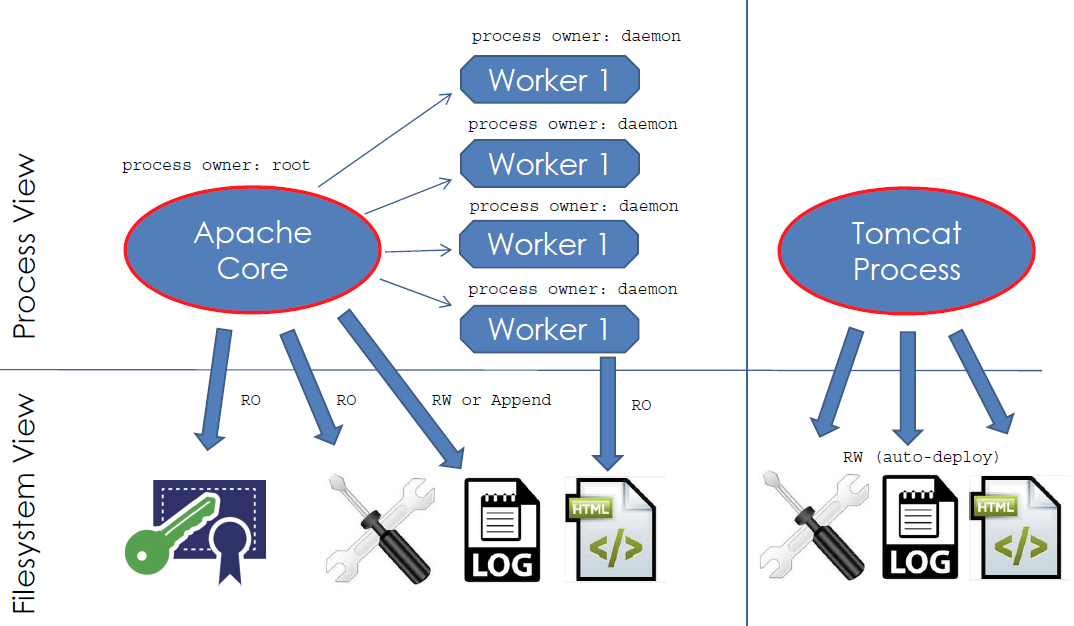
\includegraphics[width=\textwidth]{./img/apache_tomcat_permissions}
	\caption{Beispiel der Berechtigungen für Apache und Tomcat}
\end{figure}

\subsubsection{Apache File Permissions}
\begin{easylist}[itemize]
	& Root sollte \textit{Owner} sein von:
	&& Konfigurationsdateien
	&& SSL Schlüssel
	&& Log Dateien
	&& Html Dateien
	& Der Eigentümer des Apache Prozess sollte nur \textit{ReadOnly} benötigen von:
	&& Html Dateien
\end{easylist}

\subsubsection{Tomcat File Permissions}
Tomcat benötigt mehr Berechtigungen wegen seiner Deployment-Architektur. Der Eigentümer des Tomcat-Prozess benötigt \textit{ReadWrite} für Remote Deployment / Konfiguration und Load Balancing.

\subsection{Privilege Escalation}
Darunter versteht man die Möglichkeit, die Berechtigungen des aktuellen Prozesses so zu verändern, dass man Zugriff auf andere, geschützte Elemente erhält. Dazu können z.B. Bugs in SetUID-Tools verwendet werden.\\

Auch CRON kann gefährlich sein, da die Prozesse als Root gestartet werden. Wenn ein CRON-Skript "'world-writeable"' ist, kann ein Angreifer leicht den Code ändern und mit höchsten Berechtigungen ausführen lassen.

\subsection{Network Hardening}
\textbf{Nur die nötigsten Dienste} sollten auf Anfragen von aussen reagieren. Alle anderen müssen an \textit{localhost} gebunden sein. Alternativ kann auch eine \textbf{Firewall} dafür eingesetzt werden.\\
Dienste wie UPNP, Bonjour / Zeroconf und DLNA sollten aufgrund ihrer grossen \textit{Attack-Surface} auch deaktiviert werden. Dies kommt daher, dass oftmals die Geräte unzureichende Authentifizierungsmechanismen implementiert haben.\\

Es wird in den Folien auch von der \textbf{Verwendung von IPv6 abgeraten}.\\

\textbf{ICMP-Redirects deaktivieren}, um MITM-Attacken vorzubeugen.\\

Eine Analyse mittels Nmap oder \fnurl{https://cisofy.com/lynis/}{Lynis von Cisofy} kann helfen, Schwachstellen aufzudecken.

\subsection{DB Hardening}
Wie auf das Dateisystem trifft das Prinzip \textbf{Least Privileges} auch auf die Datenbank zu. Der in der Anwendung hinterlegte Benutzer darf nur auf seine Datenbanken Berechtigungen erhalten. Es können in einer Anwendung auch mehrere Benutzer mit unterschiedlichen Berechtigungen hinterlegt werden. So z.B. ein Benutzer nur mit \textit{SELECT}-Permissions für Abfragen, \textit{INSERT} und \textit{UPDATE} für Bestellungen und \textit{CREATE}, \textit{DELETE} für den DB-Admin.\\

\textbf{Keinesfalls sollte ein Applikations-User \textit{GRANT}-Permissions erhalten.}

\subsection{SSL/TLS: SSL-Cipher-Suite-Hardening}

\subsubsection{Apache SSL Cipher Hardening}
Der Nachteil des Apache SSL Cipher Hardening ist, dass der Benutzer eine unfreundliche Fehlermeldung erhält, falls er keine der geforderten SSL Cipher unterstützt.
\begin{easylist}
	& SSLProtocol
	&& Definiert, welche Protokolle akzeptiert werden
	& SSL-Cipher-Suite-Hardening
	&& Definiert, welche SSL-Cipher akzeptiert werden
	& SSLHonorCipherOrder
	&& Die Server SSL-Cipher Suit hat mehr Priorität als die des Clients.
\end{easylist}
\begin{figure}[H]
	\centering
	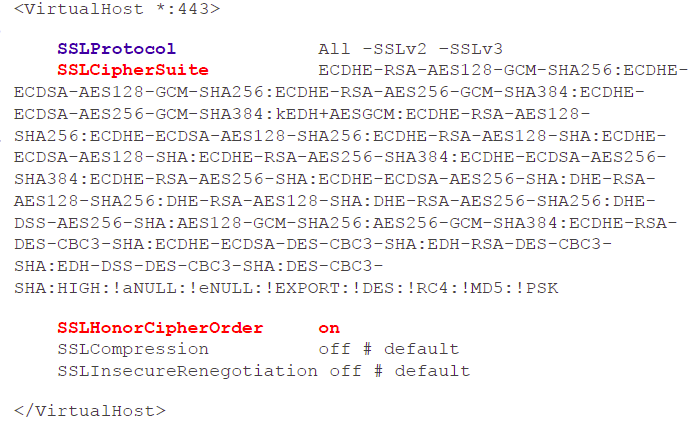
\includegraphics[width=0.8\textwidth]{./img/apache_ssl_configuration.png}
	\caption{Apache SSL Configuraiton}
\end{figure}

\subsubsection{Apache SSL Cipher Forwarding}
Der Vorteil dieser Variante ist, dass auch ältere Browsers sich mit der Applikation verbinden können, da der Apache alle Ciphers akzeptiert.\\

Apache leitet die SSL Informationen zur Applikation via \textit{mod\_headers} weiter, welche dann den Entscheid für die entsprechende SSL Cipher Suit macht.
\begin{easylist}
	& \textbf{Applikation muss die Cipher prüfen}
	& Bei Änderungen oder neuer Cipher muss die Applikation neu konfiguriert werden.
\end{easylist}